%%%%%%%%%%%%%%%%%%%%%%%%%%%%%%%%%%%%%%%%%%%%%%%%%%%%%%%%%%%%%%%%%%%%%%%%
\chapter{Introduction}\label{chap:intro}
A long-standing challenge for research in computer science is the understanding of written text and extraction of useful information from it. Text that is created by humans is often unstructured and ambiguous, whereas machine learning algorithms typically prefer fixed-length inputs and outputs. Thus, they cannot work directly with raw text directly and convert it into vectors of features.
\\
\begin{figure}
\centering 
\resizebox{0.3\textwidth}{0.25\textwidth}{      

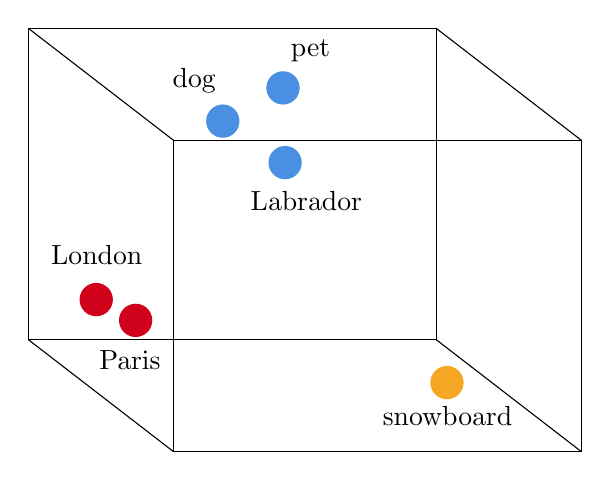
\begin{tikzpicture}[x=0.75pt,y=0.75pt,yscale=-1,xscale=1]
%uncomment if require: \path (0,300); %set diagram left start at 0, and has height of 300

%Shape: Rectangle [id:dp09766223150045761] 
\draw   (53,38) -- (249.5,38) -- (249.5,188) -- (53,188) -- cycle ;
%Shape: Rectangle [id:dp15444454726665247] 
\draw   (123,92) -- (319.5,92) -- (319.5,242) -- (123,242) -- cycle ;
%Straight Lines [id:da41180023590596115] 
\draw    (53,38) -- (123,92) ;


%Straight Lines [id:da8327746912035379] 
\draw    (53,188) -- (123,242) ;


%Straight Lines [id:da7076376732109662] 
\draw    (249.5,38) -- (319.5,92) ;


%Straight Lines [id:da531943191161679] 
\draw    (249.5,188) -- (319.5,242) ;


%Shape: Circle [id:dp5653236923369969] 
\draw  [color={rgb, 255:red, 74; green, 144; blue, 226 }  ,draw opacity=1 ][fill={rgb, 255:red, 74; green, 144; blue, 226 }  ,fill opacity=1 ] (168,66.75) .. controls (168,62.47) and (171.47,59) .. (175.75,59) .. controls (180.03,59) and (183.5,62.47) .. (183.5,66.75) .. controls (183.5,71.03) and (180.03,74.5) .. (175.75,74.5) .. controls (171.47,74.5) and (168,71.03) .. (168,66.75) -- cycle ;
%Shape: Circle [id:dp7862090364041379] 
\draw  [color={rgb, 255:red, 74; green, 144; blue, 226 }  ,draw opacity=1 ][fill={rgb, 255:red, 74; green, 144; blue, 226 }  ,fill opacity=1 ] (169,102.75) .. controls (169,98.47) and (172.47,95) .. (176.75,95) .. controls (181.03,95) and (184.5,98.47) .. (184.5,102.75) .. controls (184.5,107.03) and (181.03,110.5) .. (176.75,110.5) .. controls (172.47,110.5) and (169,107.03) .. (169,102.75) -- cycle ;
%Shape: Circle [id:dp04017773076556641] 
\draw  [color={rgb, 255:red, 74; green, 144; blue, 226 }  ,draw opacity=1 ][fill={rgb, 255:red, 74; green, 144; blue, 226 }  ,fill opacity=1 ] (139,82.75) .. controls (139,78.47) and (142.47,75) .. (146.75,75) .. controls (151.03,75) and (154.5,78.47) .. (154.5,82.75) .. controls (154.5,87.03) and (151.03,90.5) .. (146.75,90.5) .. controls (142.47,90.5) and (139,87.03) .. (139,82.75) -- cycle ;
%Shape: Circle [id:dp3593472220907403] 
\draw  [color={rgb, 255:red, 245; green, 166; blue, 35 }  ,draw opacity=1 ][fill={rgb, 255:red, 245; green, 166; blue, 35 }  ,fill opacity=1 ] (247,208.75) .. controls (247,204.47) and (250.47,201) .. (254.75,201) .. controls (259.03,201) and (262.5,204.47) .. (262.5,208.75) .. controls (262.5,213.03) and (259.03,216.5) .. (254.75,216.5) .. controls (250.47,216.5) and (247,213.03) .. (247,208.75) -- cycle ;
%Shape: Circle [id:dp42932079750070606] 
\draw  [color={rgb, 255:red, 208; green, 2; blue, 27 }  ,draw opacity=1 ][fill={rgb, 255:red, 208; green, 2; blue, 27 }  ,fill opacity=1 ] (78,168.75) .. controls (78,164.47) and (81.47,161) .. (85.75,161) .. controls (90.03,161) and (93.5,164.47) .. (93.5,168.75) .. controls (93.5,173.03) and (90.03,176.5) .. (85.75,176.5) .. controls (81.47,176.5) and (78,173.03) .. (78,168.75) -- cycle ;
%Shape: Circle [id:dp1106554795442356] 
\draw  [color={rgb, 255:red, 208; green, 2; blue, 27 }  ,draw opacity=1 ][fill={rgb, 255:red, 208; green, 2; blue, 27 }  ,fill opacity=1 ] (97,178.75) .. controls (97,174.47) and (100.47,171) .. (104.75,171) .. controls (109.03,171) and (112.5,174.47) .. (112.5,178.75) .. controls (112.5,183.03) and (109.03,186.5) .. (104.75,186.5) .. controls (100.47,186.5) and (97,183.03) .. (97,178.75) -- cycle ;

% Text Node
\draw (133,63) node   {dog};
% Text Node
\draw (189,49) node   {pet};
% Text Node
\draw (187,121) node   {Labrador};
% Text Node
\draw (255,225) node   {snowboard};
% Text Node
\draw (86,147) node   {London};
% Text Node
\draw (102,198) node   {Paris};


\end{tikzpicture}



}
\caption{An example of dense vector representation of words in a 3-dimensional space, that maps words with similar meaning to nearby points.}
\label{fig:vsmodels}
\end{figure}
Traditional \emph{Natural Language Processing} (NLP) systems treat words as atomic units, represented as vectors, where each word is treated as a one-hot vector (with $1$ in a single position and zero for the rest) to the size of the vocabulary. These vectors are sparse and orthogonal, and therefore, contain no notion of similarity among themselves. For example, if a user is searching for \emph{``Heidelberg Hotel''}, documents containing \emph{``Heidelberg Motel''} are to be disregarded since the dot product of the one-hot vectors of \emph{``Hotel''} and \emph{``Motel''} is zero. On the other hand, distributed vector space models represent words in a continuous vector space, where a word is represented by its relation to the surrounding words. These models are based on the idea that similar words tend to occur in a similar context or as the British linguist J.R. Firth said:\\ \\
\noindent
\say{You shall know a word by the company it keeps.} (J.R. Firth 1957)\\
\\
These distributed representations or so-called \emph{wod embeddings}, map words of a vocabulary to a dense vector, such that words with closer meanings are mapped to the nearby points and the similarity between them is computed based on their distance in the embedding space. An example of the embedding space is illustrated in Figure~\ref{fig:vsmodels}, where the vectors of \emph{``dog''},  \emph{``pet''} and, \emph{``labrador''} are mapped to nearby points and are farther away from unrelated words like \emph{``snowboard''}.\\
Learning dense vector representations of words dates back to $2000$ in the paper by Bengio et al., where they presented a neural probabilistic language model~\brackettext{\cite{DBLP:conf/nips/BengioDV00}}. The first simple and scalable algorithm, however, is \emph{word2vec} presented by Mikolov et al., where the aim is to capture the meaning of a word based on the surrounding context\brackettext{\cite{DBLP:journals/corr/abs-1301-3781}}. There exist numerous variations of this model, from taking the character level information into account ~\brackettext{\cite{DBLP:journals/tacl/BojanowskiGJM17}} to incorporating the statistics of the whole corpus, namely the \emph{GloVe} model~\brackettext{\cite{DBLP:conf/emnlp/PenningtonSM14}}. The GloVe model in particular, speeds up the learning and when trained on a large corpus tends to generate more promising results on downstream tasks such as named entity recognition.\\
Methods based on word2vec, despite being good at capturing semantics, have some drawbacks. They treat all words equally as terms and cannot be directly used to represent named entities. \emph{Named Entities} (NEs) refer to proper names or nouns and numerical expressions, such as dates and quantities~\brackettext{\cite{DBLP:conf/lrec/ToralMM08}}.
Many NLP tasks either depend on or use named entities as input. Identifying these references and classifying them has given rise to named entity recognition and disambiguation tasks. They are also extensively used in \emph{Information Retrial} (IR) and search engines. Disregarding the named entities while generating a word embeddings creates several challenges for downstream tasks that use them as input. Named entities often contain compound words and phrases that if not grouped together from the start, result in ambiguous and unclear representations. Although some work has been done on embedding phrases~\brackettext{\cite{DBLP:journals/tacl/HillCKB16,DBLP:conf/acl/YinS14}} or combining compound words after training with averaging, adding, or multiplying~\brackettext{\cite{DBLP:conf/eacl/DurmeRPM17,DBLP:journals/cogsci/MitchellL10}}, none of these focus on entities. The models that do focus on embedding entities, however, are designed for task specific applications, such as named entity disambiguation~\brackettext{\cite{DBLP:conf/conll/YamadaS0T16,DBLP:conf/conll/FangZWCL16}}. These models are not only task-specific but also are focused on learning representations of \emph{knowledge base} (databases containing information about named entities and their relation in a collection of documents) and do not focus on learning general purpose embedding of entities and words directly form a textual corpus.\\
A term-based model fails to distinguish between entity homographs such as  \emph{``Paris''},  which can refer to the French capital, the American heiress, or even the Trojan prince. Moreover, it cannot recognize compound word, as any word separated by space is considered its own token, whereas many companies and actors names consist of two word that not necessarily separate.  In a term-based model, if an entity is repeated several times with different names, each name is treated independently that result in loss of valuable context information for the entity. Another drawback of term-based models is their inability to deal with date information. There exist multiple form of representing date and time in text, e.g, $1$ January $1998$ or $1998$-$01$-$01$T$15$:$53$:$00$. Most models disregard any numeric information in text and limit themselves to a certain alphabet, with the exception of a few studies that try to add a temporal dimension to a paragraph or word embeddings, still they mostly focus on how the embeddings evolve or change with time and do not achieve a vector representation of dates~\brackettext{\cite{DBLP:conf/coling/MirzaT16a,DBLP:conf/ecir/YoonMWLK18}}.  \\
Another drawback of classical word embeddings in general is the lack of interpretability. In many cases, the semantic structure is heterogeneously distributed across the embedding dimensions, which makes interpretation challenging. Recently, some research has been done to make the embedding less ambiguous~\brackettext{\cite{DBLP:journals/corr/FaruquiTYDS15,DBLP:conf/emnlp/ParkBO17,DBLP:conf/aaai/SubramanianPJBH18}}. However, none of them show any insight about possible entity relations and most are applied as a post-processing step to the trained embedding. They offer no solution to learn the embeddings as an interpretable component during training time or an efficient method that can produce interpretable embeddings based on the entities surrounding a word. It is still unknown, what the implications are if a model predicts, for example,  \emph{``London''} and \emph{``Berlin''} as similar. Dense vectors representing these words do not show the reason behind their similarity. It is not obvious, whether they both appeared in the same context location-wise, e.g., both are capitals and are situated in Europe or because they share the same organizations, e.g., many companies planned to move their offices from London to Berlin after the Brexit and are mentioned in the same context. \\
Since named entities play an important rule in many NLP and IR tasks, a more intelligent representation of them enhances the performance of systems that utilize them as input features. Word embeddings are used for named entity recognition, linkage, and entity ranking~\brackettext{\cite{DBLP:conf/conll/EshelCRMYL17,DBLP:conf/nodalida/Siencnik15,DBLP:conf/icassp/MaKBK16,DBLP:conf/naacl/LampleBSKD16}}, where a unique and unambiguous representation of entities can boost their performance.
Search engines, query expansion~\brackettext{\cite{DBLP:conf/acl/0001MC16,DBLP:conf/cikm/KuziSK16}}, and document ranking~\brackettext{\cite{DBLP:conf/sigir/ZamaniC17}} that utilize named entities can also benefit from a joint representation of words and entities.
On the other hand, annotating the text with named entities, requires extensive pre-processing, from sentence splitting and tokenization to part-of-speech tagging. Not only are these steps prone to errors, but also the task of recognizing and classifying entities, even with the state-of-the-art tools, is far from perfect. Therefore, naively applying the word embedding methods to entity annotated text might cause more problems than benefits. It is important that the drawbacks of such an approach alongside its advantages are analysed. 

% BR
%
% Good introduction, but it gets quickly bogged down in details.
% Everything important is there but you should rather present a single
% use case and expand from there. The idea of interspersing related work
% within the introduction is nice, but this could also become a separate
% section.

%%%%%%%%%%%%%%%%%%%%%%%%%%%%%%%%%%%%%%%%%%%%%%%%%%%%%%%%%%%%%%%%%%%%%%%%
\section{Objective and Contributions}
In this thesis, we address the problems of term-based models for generating embeddings for named entities as well as terms using an annotated corpus. In addition, to further analyse the importance of each entity type we experiment with faceted embeddings as a method to better understand the semantic structures and increase the interpretability of vector space models. Therefore, this thesis discusses two main models, one the entity and term embeddings and one for the faceted model. Below, we will discuss the contribution of each separately.\\
By analysing the entity-based models we make the following contributions:
\begin{itemize}
\item We apply the state-of-the-art word embedding methods on an annotated corpus to jointly train embeddings for terms and entities. 
\item We use graph embedding techniques to embed the nodes of a co-occurrence graph, extracted from an annotated text as an alternative means of obtaining entity embeddings. 
\item We evaluate both of our models against well-established word embedding methods on a set of intrinsic evaluation tasks. 
\item Since a few test datasets contain any entities, we create some of our own, to better analyse the effect of entity annotation. 
\item Through visualization and experimental analysis, we investigate the underlying semantics that entity embeddings capture,  and discuss the implications for entity-centric downstream tasks.
\item By comparing the entity-based and term-based methods, we identify their strengths, weaknesses and application scenarios.
\end{itemize}
To further analyse the impact of different types of entities on a word semantics and to make the embeddings more interpretable, we introduce faceted embeddings. With the faceted model, we make following contributions: 
\begin{itemize}
\item We modify well-established word embedding techniques to include separable parts, where each part of the embedding corresponds to a specific types of entities. 
\item We use graph embedding techniques on a co-occurrence graph extracted from an annotated corpus to examine the relation of each word to the neighbours of a specific type. By embedding the nodes of such a graph we introduce an alternative way to achieve the faceted model.
\item We evaluate our faceted models against the term-based methods on raw text, on a set of intrinsic evaluation tasks. 
\item Since separate parts of faceted embeddings divide the embedding space into the different type of entities available in text, we investigate the effect of each type on intrinsic tasks. 
\item By visualizing the embedding parts separately, we explore potential use cases and the underlying semantics of such models.   
\end{itemize}

% BR: A good section, but the structure should be more succinct. When
% this is read (by the grader), I should immediately see what the
% objectives were and how they have been achieved. Maybe a different
% layout with 'at-a-glance' contributions would be helpful here. It is
% good that you use concrete examples, but there should be a brief
% summary about them.


%%%%%%%%%%%%%%%%%%%%%%%%%%%%%%%%%%%%%%%%%%%%%%%%%%%%%%%%%%%%%%%%%%%%%%%%
\section{Overview of the Thesis Structure}
The remainder of this thesis is structured as follows: 
In Chapter~\ref{chap:background},  we discuss the background information required for the model and related work, with a brief introduction to the basics of NLP and neural networks. This discussion is followed by, an explanation of well-established word embedding and graph embedding methods, which are the base of the entity-based models. In Chapter~\ref{chap:entity}, we present two types of models for learning terms and entity embeddings jointly on an annotated corpus. One method focuses on learning the vector representation from a textual corpus, while the other method requires a co-occurrence graph extracted from the annotated text.
Chapter~\ref{chap:faceted} contains an in-depth definition of the faceted embeddings, where different models are proposed based on the input data (textual or graph-based). 
In Chapter~\ref{chap:eval}, we present the test cases and evaluation results. The entity embeddings and faceted models are analysed using visualizations and also tested against well-known analogy, word similarity and categorization datasets. The work is closed with a conclusion and outlook on possible future work in Chapter~\ref{chap:concl}. 


% BR: Very nice in total. I would recommend the following, though:
%  - make the claims more concise and precise
%  - formulate the objectives and how this was achieved.
%  - ideally, you can formulate both at the same time and place
%  - for example, I had 'Contributions' in my dissertation as well, you
%    may want to look at these (text me if you have troubles finding
%    that)
